\chapter{Theoretical Framework}
\label{chapter:theoretical-framework}


In this chapter is described the theoretical concepts needed to understand the work developed during the research's execution.


\section{Room Impulse Response}

An acoustic impulse is a sharp, narrow pulse whose spectrum is composed of a uniform distribution of all frequencies. The mathematical Dirac delta function \( \delta(t)\) is used to represent this kind of impulse. In enclosed spaces, the sound waves generated by an impulse travel, reflect, and refract on the walls delimiting the space. A microphone measuring the environment first receives the direct-path sound, which travels from the source directly to the microphone, followed by the early reflections and finally by a series of pulses called late-field reverberation, as shown in Figure \ref{fig:RIR}. The direct path, early reflections, and reverberation correspond to the response of the enclosed space to an acoustic impulse and are physically defined by the geometry and materials of the environment \cite{RIR01}.

The Room Impulse Response (RIR) is, by definition, the transfer function of a sound wave that travels through the space from its source to the microphone. A microphone records the convolution of the emitted sound with the corresponding RIR \cite{RIR02}, as shown mathematically in Equation \ref{eqn:sound} with \(g(t)\) representing the recorded signal, \(h(t)\) the RIR, and \(x(t)\) the emitted sound. Therefore, any sound generated at one point and received at another inside a room contains the effects of the RIR of the environment.    

\begin{equation*}
\label{eqn:sound}
g(t)=h(t)*x(t)= \int_{-\infty}^{\infty} h(t)x(t-s)ds \tag{1}
\end{equation*}


\begin{figure} [hbt!]
	\begin{center}
		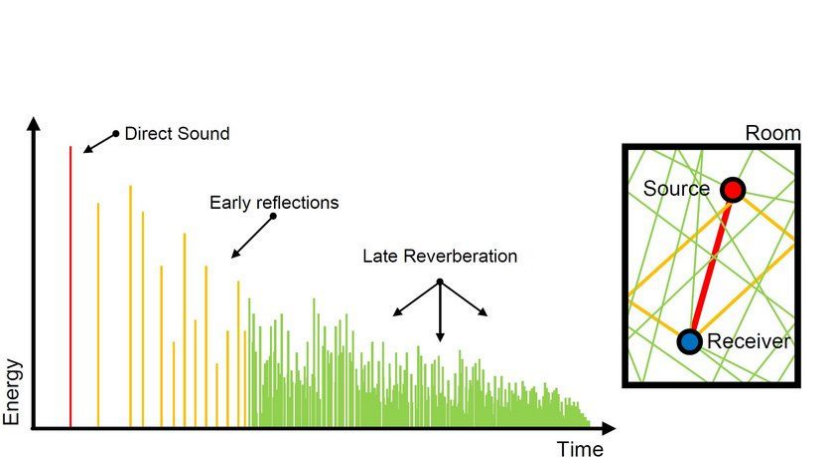
\includegraphics[width=1\columnwidth]{../img/RIR.png}
		\caption{Room Impulse Response and the geometrical room representation \cite{RIR03}.}
		\label{fig:RIR}
	\end{center}
\end{figure}


\section{Acoustic Beamforming}

In many spatial omnidirectional data transfer contexts, not only the information carried in the medium is important: the source from which the signal is generated also provides valuable information for properly analyzing the incoming data. Beamforming is a spatial filtering technique that aims to estimate the direction of arrival of a signal, even in the presence of noise and other interference in the propagation medium \cite{BEA01}. In acoustics, an array of microphones is used to capture spatially propagated signals arriving from a certain direction and to process them in order to investigate the acoustic sources \cite{BEA02}.
\label{section:Concept2}

\subsection{Microphone Array}

A microphone array combines the signals of multiple omnidirectional microphones in such a way that it captures sound from a specific direction while rejecting sound from other directions \cite{MA01}. The shape and dimensionality of the arrangement depend on the application. The simplest form consists of two microphones separated by a distance \(D\), as shown in Figure \ref{fig:micdipole}. The value of \(D\) is the minimum distance for a given frequency at the sound speed \(c\), and its calculation is shown in Equation \ref{eqn:ddipole}. When the input signals are simply added together for a given frequency \(f\), this arrangement captures sound coming from \(\pm\)90 degrees and rejects sound arriving from 0 and 180 degrees. In a microphone array, a higher number of microphones results in greater gain in the desired direction as well as greater attenuation of sound coming from the sides of the array \cite{MA02}.

\begin{figure}[hbt!]
	\begin{center}
		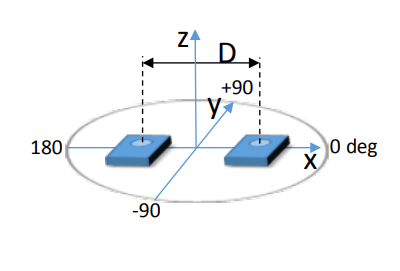
\includegraphics[width=9cm, height=7cm]{../img/mic_dipole.png}
		\caption{Microphone array in binaural arrangement \cite{MA01}.}
		\label{fig:micdipole}
	\end{center}
\end{figure}

\begin{equation*}
\label{eqn:ddipole}
D=\frac {1}{4} \frac {c}{f}\tag{2}
\end{equation*}

\subsection{Beamforming Pipe}

\subsubsection{Delay-and-Sum Beamforming Technique}

Beamforming is based on the physical principle that an acoustic wave originating at a particular location in space travels and arrives at each sensor at a different time, defined by the distance between the single source and each sensor. The result of adding all these signals depends on the phase relationship between them, so it is possible to control the delay of each signal to constructively add those from a particular location while, at the same time, destructively canceling those originating in other regions \cite{BEA01}. Mathematically, the beamforming formula is shown in Equation \ref{eqn:beamforming}, where \(L(t,S_0)\) is the beamforming output and \(p_m\) is the microphone output for a signal originating at \(S_0=(x_0,y_0,z_0)\) and captured by a microphone located at \(S\). All the signals are summed together and divided by the total number of microphones \(M\) in the array.

\begin{equation*}
\label{eqn:beamforming}
L(t,s_0)=\frac {4\pi}{M} \sum_{m=1}^M pm(s_0,t+t_0)|S-S_0| \tag{3}
\end{equation*}

%\subsubsection{Deconvolution}
%In real applications, the beamforming output comprises the acoustic signal convolved with the microphone array response. The deconvolution principle assumes that %the recorded signal \(r(t)\) is the convolution of the sound \(g(t)\) (as shown in Equation \ref{eqn:sound}) and a transfer function for the array, which %represents the array response to a given source \cite{BEA01}. The Point-Spread Function (PSF) is the array response to a monopole placed in front of the array. %The PSF provides the information required to obtain the array transfer function needed for deconvolution, which extracts the sound free of the distortion created %by the array.

\subsubsection{Post-Filtering}

Considering that the signal measured by each microphone is the sum of the sound and the noise, and that the noise is uncorrelated between microphones and with the beamforming output signal, the beamforming output can be further enhanced by selectively filtering the resulting signal based on the cross-spectral densities between channels in the microphone array \cite{BEA02}.


\section{Time Series Transformation into Images}

Given a time series, it is sometimes desirable to apply certain transformations that provide a more compact representation of the data or highlight specific properties and attributes of it. Transforming a time series into an image involves converting vectors into matrices using a transformation criterion that maps values from one domain to another. One example is the conversion of audio signals into spectrograms or log-mel spectrograms, which provide a time-frequency representation of the signal. In machine learning applications, these image-like representations can be used as input to convolutional neural networks and other image-based models, enabling the extraction of meaningful features from time series data.

\subsection{Log-Mel Spectrogram}

Spectrograms are widely used in audio and speech processing, as well as in other fields where time-varying signals are analyzed \cite{spectrogramns1}. A spectrogram is a visual representation of the spectrum of frequencies of a signal over time. It is obtained by dividing the signal into overlapping segments, applying a window function to each segment, and computing the Fourier transform to obtain the frequency content. The resulting magnitude is then plotted as a function of time and frequency, providing a time-frequency representation of the signal.

\subsection{Log-Mel-Scale}

The mel scale is a representation of how people perceive audio pitches. It is based on the ability of humans to judge equal distances between pitches. Pitch, in acoustics, is the perceptual quality that allows sounds to be ordered from low to high by frequency, which is what the human mind does when processing tones \cite{melscale}.

The conversion from frequency to the mel scale is given by Equation \ref{eqn:mel}.


\begin{equation}
\label{eqn:mel}
m(f) = 2595 \log_{10}\left(1 + \frac{f}{700}\right) = 1127 \ln\left(1 + \frac{f}{700}\right)
\end{equation}

For the discretization of the mel frequencies, the continuous mel scale is filtered using a bank of triangular bandpass filters, each representing a specific range of mel values. The canonical number of filters is 128 in applications with complex environmental audio tasks, in order to preserve fine spectral cues \cite{melscale}.


\section{Convolutional Neural Network}

A Convolutional Neural Network (CNN) is an artificial neural network architecture used to analyze and learn from visual data, commonly presented in the form of images. In its simplest form, the structure is composed of three building blocks: the convolution layer, the pooling layer, and the fully connected layer. Figure \ref{fig:fullcnn} shows an example of how these blocks are connected to analyze an image stage by stage in order to determine the structural condition of an aircraft fuselage.


\subsection{Convolution operation}

Convolution is a common operation used in image filtering to denoise or detect features. A filter, also called a convolution kernel, is applied to all locations of the image to produce a new filtered image \cite{convdef}. A filter \(W\) of dimension \(K \times L\) with weights \(w_{k,l}\) can be convolved with a given 2D image \(X\) of dimension \(I \times J\) with pixels \(x_{i,j}\) to obtain a filtered image \(X*W\). The convolution process over the image can be mathematically written as:

\begin{equation}
\label{eqn:conv}
(w*x)_{i,j}=\sum_{k=-K/2}^{K/2}\sum_{l=-L/2}^{L/2} w_{k,l}x_{i+k,j+l} \tag{5}
\end{equation}
\\

\begin{figure}[hbt!]
	\begin{center}
		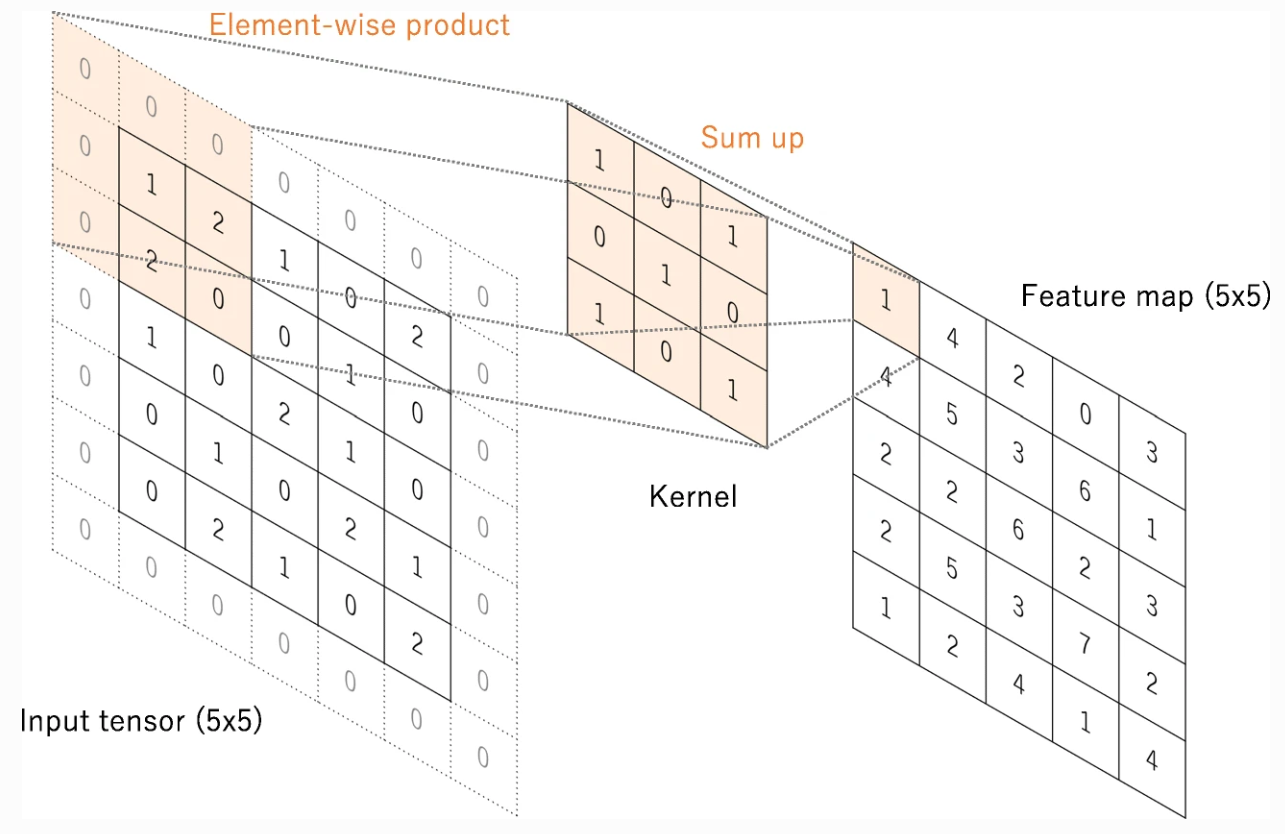
\includegraphics[width=12cm, height=9cm]{../img/convolution.png}
		\caption{Convolution operation over a tensor of 5x5 with zero padding and a stride of 1, resulting in a feature map of 5x5 \cite{convpadd}.}
		\label{fig:conv}
	\end{center}
\end{figure}


The convolution operation in Equation \ref{eqn:conv} does not allow the center of the kernel to overlap the edges of the image, resulting in a reduction in the size of the output feature map. Padding increases the input size by adding extra rows and columns around the outermost elements on each side of the image in order to compensate for this dimensional reduction \cite{convpadd}. In practice, as shown in Figure \ref{fig:conv}, the kernel is applied across the input one step at a time. An element-wise operation is performed at each location and the results are summed to obtain the output. The kernel is then moved to the next location to filter another segment of the input. The size of the kernel displacement is given by the stride, which defines the distance between two successive kernel positions.
\\



\subsection{Pooling}
Pooling is a dimension reduction technique in which an input map is spatially reduced while keeping the most important features that were filtered or learned. The pooling operation reduces or collapses a subregion to a smaller dimension, helping the learned representation become more invariant to small length-scale perturbations \cite{polling}.

Two common pooling techniques are max-pooling and average-pooling. For a defined pooling window, max-pooling considers only the maximum value, whereas average-pooling calculates the average of the values inside the window, as shown in the example in Figure \ref{fig:avg_max_p}.

\begin{figure}[hbt!]
	\begin{center}
		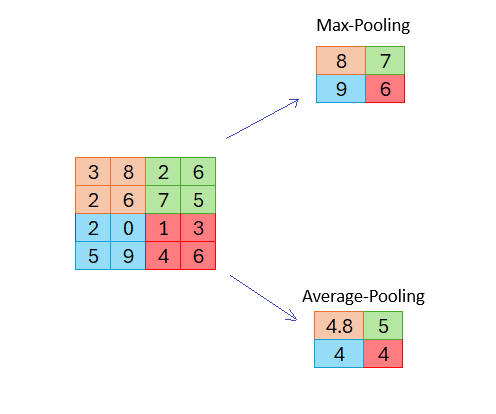
\includegraphics[width=10cm, height=8cm]{../img/avg_max_pooling.png}
		\caption{Pooling escalation with average pooling and max-pooling.}
		\label{fig:avg_max_p}
	\end{center}
\end{figure}

\subsection{Fully connected layer}

The final stage in a CNN is a fully connected layer. This layer is responsible for classifying the features extracted by the previous layers. Figure \ref{fig:fullcnn} shows an example of a CNN for aircraft structural health classification, with its fully connected layer located at the output of the network.


\begin{figure}[hbt!]
	\begin{center}
		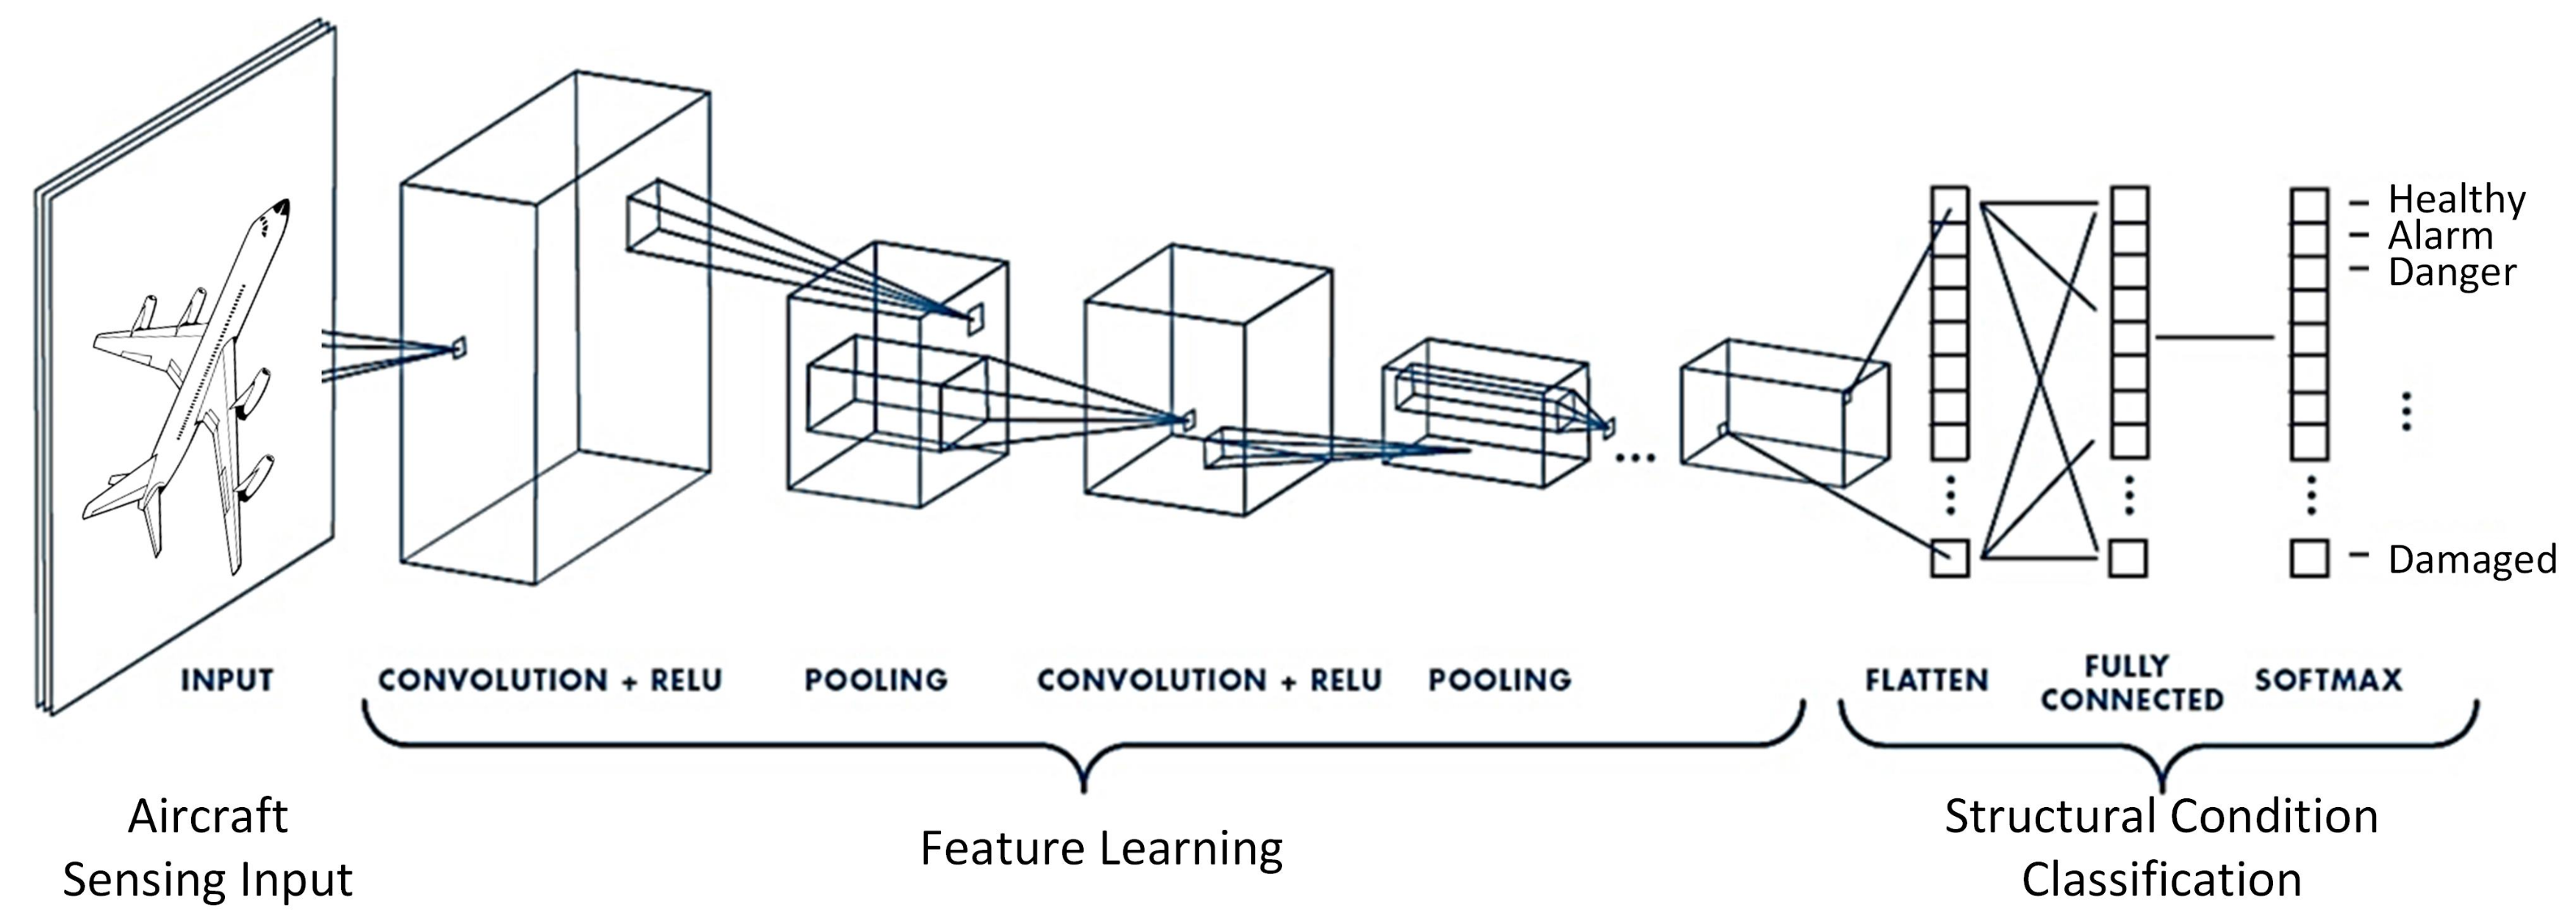
\includegraphics[width=15cm, height=6cm]{../img/CNN full.png}
		\caption{Architecture of Convolutional Neural Network for aircraft structural health monitoring \cite{cnnimg}.}
		\label{fig:fullcnn}
	\end{center}
\end{figure}

\section{Echo State Network}

An Echo State Network (ESN) is a recent paradigm in recurrent neural networks known as Reservoir Computing (RC). In RC, the reservoir is the recurrent part of the network and has the particularity of not being trained. Because the reservoir skips training, the network avoids the computationally expensive gradient-descent training of recurrent networks. Instead, the recurrent network is defined in such a way that it can transform input signals into values in a high-dimensional state space. The state of the reservoir can be processed by a simple fully connected readout network trained to map the reservoir state to a desired output \cite{RC1}.

In the ESN, the reservoir is a randomly created RNN whose weights remain unchanged. This RNN is excited by an input signal, and its future state is a function of the current input and the history of the reservoir. The result is generated by training a simple feed-forward network to output the target value. Figure \ref{fig:imgRC1} \cite{RC1} shows a comparison of a traditional RNN and RC. In RC, the bold arrows exemplify the weight changes resulting from the training process, which is performed only at the output layer of the network.



\begin{figure}[hbt!]
	\begin{center}
		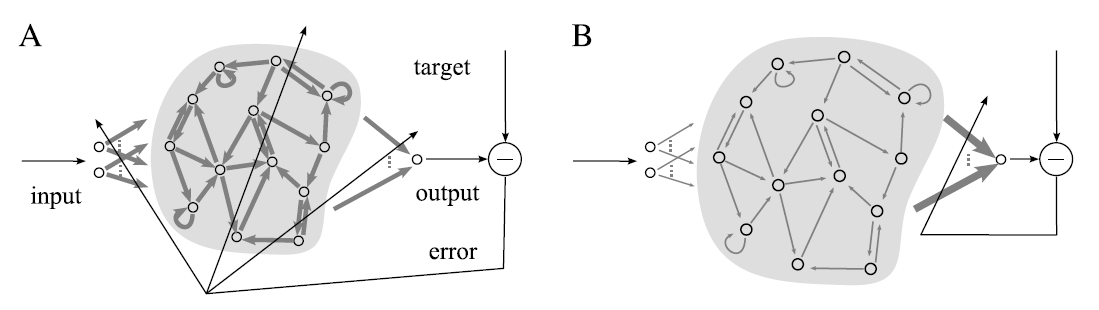
\includegraphics[width=14cm, height=4cm]{../img/imgRC1.png}
		\caption{Comparison of B) RC vrs A) traditional RNN, the bold arrows are weights that change during training \cite{RC1}.}
		\label{fig:imgRC1}
	\end{center}
\end{figure}


\subsection{Formalism of ESN}

A formal description of an ESN, given in \cite{RC2}, defines an ESN that receives a time series input \(U(t) \in R^{D \times 1}\), where the state of the reservoir is denoted by \(X(t) \in R^{N \times 1}\) and the output by \(y(t) \in R^{M \times 1}\). The weights for the stages are \(W_{in} \in R^{N \times D}\) for the input, \(W_{res} \in R^{N \times N}\) for the reservoir, and \(W_{out} \in R^{N \times M}\) for the output. The equations for the internal state of the reservoir and the output are shown in Equation \ref{eqn:RCform1}. The reservoir state depends on the input value at time \(t\) and the previous state of the system. The output can be obtained by training to solve a linear regression problem.

\begin{equation}
\label{eqn:RCform1}
\tag{6}
\begin{split}
x(t)&=f(W_{in}U(t)+W_{res}x(t-1)) \\
y(t)&=W_{out}x(t)
\end{split}
\end{equation}

There is an important property that the reservoir should meet to ensure that its dynamics are capable of forgetting the initial transient state \cite{ESP_RC}. The Echo State Property (ESP) states that a network with state transition function \(F\) has the echo state property if, for each input sequence \(U=[u(1),\dots,u(N)]\) and all pairs of initial reservoir states \(x, x'\), Equation \ref{eqn:eqESP} holds.

\begin{equation}
\label{eqn:eqESP}
||F(U,x)-F(U,x')|| \to 0 \: as \: N \to \infty  \tag{7}\\
\end{equation}
\\

To ensure the existence of the ESP, \(W_{res}\) must meet a necessary condition and a sufficient condition, defined as follows:

\begin{equation}
\label{eqn:ESP2}
\tag{8}
\begin{split}
ESP& \Rightarrow \rho(W_{res}) < 1\\
\bar \sigma(W_{res})<1 & \Rightarrow ESP 
\end{split}
\end{equation}
\\

where \(\rho(W_{res})\) is the spectral radius of \(W_{res}\) and \(\bar \sigma(W_{res})\) is its largest singular value. Thus, from Equation \ref{eqn:ESP2}, if \(\rho(W_{res})\) and \(\bar \sigma(W_{res})\) are less than one, the ESP is satisfied and the reservoir dynamics will behave correctly.




\section{Related Work}
The related work in acoustic processing for object recognition and classification can be divided into two categories based on where the sound originates. An approach is considered passive sensing if the sound stimulus originates directly in the system. Conversely, if the sound is an external stimulus that interacts with the environment before being sensed, the approach is active sensing.

\subsection{Passive Acoustic Sensing and Analysis}   

\subsubsection{Acoustic Imaging}

An acoustic image is a sound intensity map that highlights the location of different sound sources in a two-dimensional plane. An acoustic camera takes this intensity map and superimposes it on an optical image to show the physical source of the sound. As shown in Figure \ref{fig:ACImg}, a microphone array is used to capture the sound, and a beamforming algorithm processes the signals to locate the direction from which the sound originates.

\begin{figure}[hbt!]
	\begin{center}
		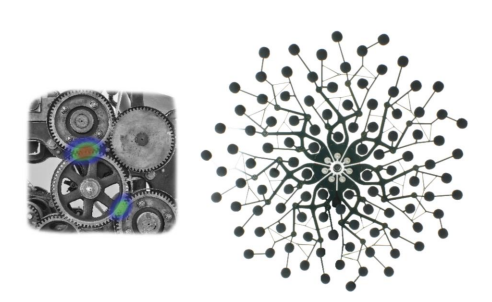
\includegraphics[width=10cm, height=6cm]{../img/acoustic image.png}
		\caption{Image on the left is an acoustic image, on the right and microphone camera used to capture the image \cite{Acamera}.}
		\label{fig:ACImg}
	\end{center}
\end{figure}

Acoustic beamforming is an extensively studied field. Different shapes and sizes of microphone arrays have been analyzed \cite{MA02}, and many techniques exist for beamforming the signals from the array \cite{BEA02}. Recent studies have focused on spherical arrays to identify multiple sound sources in three-dimensional space \cite{RWB1, RWB2, RWB3}.

\subsubsection{Acoustic Scene Classification}

Artificial Intelligence, and especially its deep learning subfield, has powered the development of new techniques to segment, analyze, and classify acoustically originated signals. Acoustic Scene Classification (ASC) uses deep learning to learn and distinguish, from audio, the context in which a recording was made. CNNs are the first choice for ASC. The images required as input to the network are obtained by processing an audio dataset to convert it into spectrograms. Using the DCASE 2016 dataset, the authors of \cite{CNNASC1} used static log-mel spectrograms and dynamic first-derivative spectrograms to build the two channels of the images used as input for training the CNN. \citeauthor{CNNASC2} in \cite{CNNASC2} used the DCASE 2017 dataset and improved the training input data through multiple versions of mel spectrograms based on binaural representation, source separation, and background subtraction. In the binaural representation, left-right and mid-side spectrograms were used instead of a mono audio representation. Source separation divides the dataset in two using harmonic-percussive sound separation algorithms, which increases the dataset by providing harmonic and percussive representations of each sound. Finally, median filtering is applied to the spectrograms to suppress steady environmental noise. The resulting multiple spectrogram versions were used to train a ConvNet architecture of eight convolution layers inspired by a VGG network. Compared with the baseline used in that work, the authors obtained an improvement in mean accuracy, from 74.8\% to 80.5\% with the various preprocessing methods described above. The work presented in \cite{ASC3} used the DCASE 2019 dataset and log-mel spectrograms to train two deep learning algorithms to perform the classification: a CNN and a Convolutional Recurrent Neural Network (CRNN). The highest recognition accuracy was obtained by the CRNN, with 90.96\%, a value superior to the 73.61\% of the CNN used as the baseline. A different objective is presented by \citeauthor{ASC4} in \cite{ASC4}, where small-footprint neural network models are investigated. The authors compared several small neural networks using the DCASE 2020 dataset and found that a 16-bit CNN with squeeze-excitation blocks, regularized with mixup and weight decay, shows the best accuracy, 66.84\%, with only 90 kilobytes of parameters.

\subsubsection{Acoustic Object Recognition}

Acoustic object recognition aims to recognize an object based on the sound it emits, whether the sound is self-generated, such as the sound produced by an air conditioner during normal operation, or external, produced in response to a stimulus, such as the characteristic sound of wood when someone knocks on a door. In the work presented by \citeauthor{AOR1} in \cite{AOR1}, a dataset was built using 30 different objects, each of which was hit with a marker pen to generate a characteristic sound that was recorded. A training set of 100 hits per object (at different locations on the object) was created, and an extra 20 hits per object were obtained for the test phase. With this dataset, a denoising autoencoder was trained to recognize the different sounds of the objects from which they originate. The recognition rate for the autoencoders was 91.50\%, a value superior to the baseline provided by a Support Vector Machine with a recognition rate of 82\%. \\
Other dataset was created by \citeauthor{AOR2_LEGO} in \cite{AOR2_LEGO}, in this case the input were LEGO objects that fall from 30cm high. The sound  of the LEGO pieces hitting the ground was used to create spectrograms to training a CNN called LegoNet in order to recognize the LEGO pieces by the sound of its free-fall impact, LegoNet achieved an accuracy of 99.21\%, a value superior to the other networks used for comparison. For robotic perception in \cite{AOR3_ROBOT} was develop a framework in which a robot can recognize the object inside a container by shaking the container and analyzing the sound. An kernel K-nearest neighbor algorithm in a open environment is used to shows the feasibility of the method. A generative physical, audio-visual synthesis pipeline is presented in \cite{AOR4}, the model takes as input the shape of an object, its material and one scene configuration, a physical engine simulate motion and collision for that particular object. An audio engine takes the shape, material and the collision information to synthesize the sound. The database generated is used in the training a two-stream CNN, one ResNet-18 for the image data, together with a SoundNet-8 for the audio data. The net demonstrated that the knowledge learned in the synthetic audio-visual dataset was transferred to real world data once it was used to infer object materials from auditory data, and estimate shape attributes from audio-visual data.

\subsection{Active Acoustic Sensing and Analysis}

\subsubsection{RIR for Room Inference}

For an enclosed space, the RIR provides a unique representation of the geometry and materials inside it. Sounds such as music and speech recorded in rooms carry this echo information and can be used to recognize the room in which the recording was made. This idea is presented in \cite{RIR05}, where the authors developed a machine learning system to identify rooms from reverberant audio samples recorded in them and achieved 85\% accuracy in the task. The work in \cite{RIR06} uses the RIR and speech data to train a model to infer the room volume from sound recorded with a single microphone. With this information, the model classified rooms into three categories (small, large, or hall) with an accuracy of 85.8\%. Using microphone arrays and analyzing the RIR obtained from them, the authors of \cite{RIR07} were able to estimate the room geometry by exploring the properties of Euclidean distance matrices, and showed that under certain conditions the first-order echoes provide a unique description of the geometry of convex polyhedral rooms. In \cite{RIR08}, an indoor positioning device is presented that uses the RIR as a ``fingerprint'' to identify the room in which the system is located. The accuracy varies depending on the type of room, ranging from 65\% for living rooms to 95\% for bathrooms. The work in \cite{RIR09} presents a dataset of RIRs in which people stood in rooms and were relocated to different positions inside them to generate samples. The authors show the potential of using machine learning approaches on the dataset for tasks related to localizing, identifying, and detecting humans in those rooms.

\subsubsection{Acoustic Object Shape Estimation}

Acoustic perception of shapes is explored in \cite{shape1}. This work proposes the use of acoustic standing waves to recognize the size and shape of a target object by analyzing the distance spectrum profile of the standing waves created by the interference between transmitted and reflected sounds. In this work, \citeauthor{shape1} were able to estimate the dimensions of a rectangular board of 1.2 m $\times$ 0.9 m, with a mean absolute error of 0.0194 m. With this result, they demonstrated that the spectrum profile encodes information about the target and can be used to estimate the shape of an object. The approach presented by \citeauthor{bat1} in \cite{bat1} resulted in the development of the Batvision system, which is capable of seeing depth and spatial layouts by listening to echoes recorded by two microphones acting as artificial ears. For Batvision, a dataset was created using mobile robots that generate acoustic chirp signals at the same time a depth image is captured. With this dataset of audio-image pairs, an adversarial discriminator was trained to generate depth images based on sound chirps. The system was capable of predicting detailed indoor scenes and obstacles with an L1 loss as low as 0.072, sometimes even outperforming a depth map created by a stereo vision algorithm. Following the findings in Batvision, the work presented in the CatChatter paper \cite{cat1} shows two separate results. First, an improved version of Batvision was developed in which an input encoder was removed from the model. This encoder processed the acoustic spectrogram before it reached the adversarial discriminator and caused spatial information from the spectrogram to be lost by the time it reached the U-Net, decreasing the inference capacity of the model. The second result presented in \cite{cat1} was a new system that uses lidar to create 3D, 360-degree depth images, together with an increase in acoustic perception from two microphones to four in order to capture echoes from all directions. The results obtained by this new method are similar to those reported for Batvision \cite{bat1}, but thanks to the 360-degree depth information and the two extra microphones, the field of prediction was four times larger than that obtained with the depth camera and two-microphone system. To detect basic shapes and deformations, acoustic sensing was used in \cite{echosense} by \citeauthor{echosense} to identify and monitor small hollow objects from the inside. The deformations of the shapes were created by generating similar shapes with altered dimensions or by blocking a certain part of the object's interior. A square wave sound signal is emitted inside the objects, and a four-microphone array records the echoes produced in the interior. Acoustic features are created from these signals, and a classifier is trained to distinguish the shape and deformation of the object under study. Their work showed that, for the objects tested, the shape can be identified with 80\% accuracy, the existence of a deformation with 100\% accuracy, and the location of the deformation with 90\% accuracy.        
